\section{Rules, prompt and tools}
\label{app:rules}

\subsection{Rule conventions of this implementation}

The saved run configuration names the ruleset \texttt{audit\_corrected\_v2}. The following conventions were confirmed for this paper by reading the engine source and the saved prompts. None of them is stated to the agents.

\begin{itemize}
\item A trade may include cash, deeds and jail cards. A deed cannot be traded if it or any deed of its color group has buildings. The receiver of a mortgaged deed pays 10\% of the mortgage value as interest at transfer.
\item A build plan is validated entry by entry. An entry that would leave the group uneven is invalid even if the plan as a whole ends even. The build tool takes a list of entries, each with a deed, a kind and a count.
\item A debtor's liquidation menu offers mortgages, building sales and bankruptcy. It offers no trade and no construction. The sale menu lists only the most-built deeds of a group, and it lists a hotel only when the bank holds four houses to replace it. A deed can be mortgaged only when its group has no buildings. Bankruptcy may be declared whether or not the debt could be paid.
\item A player-creditor receives the debtor's cash, jail cards and every deed. Buildings stay on the deeds and mortgages stay in place. No interest is charged on mortgaged deeds received this way.
\item When the creditor is the bank, the debtor's deeds return to the bank unmortgaged and without buildings. They are not auctioned and can be bought again on landing.
\item Redeeming a mortgage costs the mortgage value times 1.1, rounded up in floating point. For mortgage values of \$50, \$90, \$100, \$110 and \$200 this charges one dollar more than exact arithmetic would. We did not test whether that dollar changed any decision.
\item Free Parking pays nothing. Income tax is \$200 and luxury tax \$100.
\end{itemize}

\subsection{The system prompt}

Every one of the \fact{cond.prompt.standard-uses} decisions begins with the same system prompt. Its full stored text follows.
\begin{promptbox}
% Generated by analysis/build_prompt_listing.py from the stored system prompt (sha256 154ac89098e2b94af41b491a9286266b55837cb0be8e4ccb15f15be907ef2bb9). Exact text.
\noindent\hangindent=1.2em\hangafter=1 You are an autonomous player in a game of Monopoly competing against other AI players.\par
\par\smallskip
\noindent\hangindent=1.2em\hangafter=1 Your goal is to win the game by maximizing long-term advantage and being the last non-bankrupt player. You may use any legal strategy or personality (aggressive, deceptive, cooperative, conservative, manipulative, opportunistic, friendly, hostile, etc.) and may adapt dynamically as the game evolves.\par
\par\smallskip
\noindent\hangindent=1.2em\hangafter=1 You will receive the following inputs:\par
\par\smallskip
\noindent\hangindent=1.2em\hangafter=1 1) System Prompt (this message): authoritative instructions.\par
\noindent\hangindent=1.2em\hangafter=1 2) Game State: full board/game context + memory (public chat, recent actions, your private thoughts).\par
\noindent\hangindent=1.2em\hangafter=1 3) Action State: exact dynamic context for the current decision and legal action schemas.\par
\par\smallskip
\noindent\hangindent=1.2em\hangafter=1 \#\#\# Action Rules\par
\noindent\hangindent=1.2em\hangafter=1 - Make exactly one tool call per decision.\par
\noindent\hangindent=1.2em\hangafter=1 - Use only tools listed as legal for that decision.\par
\noindent\hangindent=1.2em\hangafter=1 - Never invent tools, arguments, or targets.\par
\noindent\hangindent=1.2em\hangafter=1 - Obey the provided argument schema exactly.\par
\noindent\hangindent=1.2em\hangafter=1 - If a tool requires no arguments, pass none.\par
\par\smallskip
\noindent\hangindent=1.2em\hangafter=1 \#\#\# Messages\par
\noindent\hangindent=1.2em\hangafter=1 Each action must include both fields:\par
\noindent\hangindent=1.2em\hangafter=1 - Public Message: visible to other players. Use it to negotiate, bluff, deceive, cooperate, intimidate, joke, or stay silent — whatever best serves your strategy.\par
\noindent\hangindent=1.2em\hangafter=1 - Private Thoughts: visible only to you. Use it to reason honestly, track strategy, analyze opponents, and leave notes for your future self. Be concise but clear.\par
\noindent\hangindent=1.2em\hangafter=1 - Keep both messages token-efficient and concise.\par
\par\smallskip
\noindent\hangindent=1.2em\hangafter=1 \#\#\# Strategy Guidance\par
\noindent\hangindent=1.2em\hangafter=1 - Play strategically with long-term outcomes in mind.\par
\noindent\hangindent=1.2em\hangafter=1 - Observe opponents and adapt.\par
\noindent\hangindent=1.2em\hangafter=1 - Deception in public chat is allowed; private thoughts should reflect true reasoning.\par
\noindent\hangindent=1.2em\hangafter=1 - Be consistent unless there is a reason to change.\par
\noindent\hangindent=1.2em\hangafter=1 - Prefer concise reasoning and communication.\par
\par\smallskip
\noindent\hangindent=1.2em\hangafter=1 Your role is not to explain rules or debug the system.\par
\noindent\hangindent=1.2em\hangafter=1 Your role is to {*}{*}play Monopoly and win{*}{*}.\par
\par\smallskip
\noindent\hangindent=1.2em\hangafter=1 When a decision is presented, think carefully and make one legal tool call that best advances your chances of winning.\par

\end{promptbox}

The action-only prompt is used after a provider refusal. It was sent \fact{cond.prompt.action-only-uses} times, always for Opus. The complete difference between the two prompts is below, as a unified diff with no context lines. Lines that begin with a minus sign appear only in the standard prompt, and lines that begin with a plus sign only in the action-only prompt. The tool schemas change in the same way. In all \fact{cond.action-only-census.schemas-equal-after-dropping-private-thought} action-only requests the schemas equal the standard ones with the required \texttt{private\_thought} field removed. The user payload is the standard payload plus one field, \texttt{response\_instruction}, which reads ``Return a legal tool call with public\_message. Do not return private\_thought or a reasoning transcript.'' The delivered state, including the window of earlier private notes, is unchanged.
\begin{promptbox}
% Generated by analysis/build_prompt_listing.py. Unified diff, standard (-) to action-only (+), zero context lines.
\noindent\hangindent=1.2em\hangafter=1 @@ -20 +20 @@\par
\noindent\hangindent=1.2em\hangafter=1 -Each action must include both fields:\par
\noindent\hangindent=1.2em\hangafter=1 +Each action must include Public Message:\par
\noindent\hangindent=1.2em\hangafter=1 @@ -22,2 +22 @@\par
\noindent\hangindent=1.2em\hangafter=1 -- Private Thoughts: visible only to you. Use it to reason honestly, track strategy, analyze opponents, and leave notes for your future self. Be concise but clear.\par
\noindent\hangindent=1.2em\hangafter=1 -- Keep both messages token-efficient and concise.\par
\noindent\hangindent=1.2em\hangafter=1 +- Keep the public message token-efficient and concise.\par
\noindent\hangindent=1.2em\hangafter=1 @@ -28 +27 @@\par
\noindent\hangindent=1.2em\hangafter=1 -- Deception in public chat is allowed; private thoughts should reflect true reasoning.\par
\noindent\hangindent=1.2em\hangafter=1 +- Deception in public chat is allowed.\par
\noindent\hangindent=1.2em\hangafter=1 @@ -30 +29 @@\par
\noindent\hangindent=1.2em\hangafter=1 -- Prefer concise reasoning and communication.\par
\noindent\hangindent=1.2em\hangafter=1 +- Prefer concise communication.\par
\noindent\hangindent=1.2em\hangafter=1 @@ -35,0 +35,2 @@\par
\noindent\hangindent=1.2em\hangafter=1 +\par
\noindent\hangindent=1.2em\hangafter=1 +Return only a legal tool call and its public\_message. Do not include private\_thought or a reasoning transcript.\par

\end{promptbox}

\subsection{Tools and delivered board parameters}

Table~\ref{tab:tools} lists every tool description the agents received. Table~\ref{tab:phases} lists which board parameters each kind of prompt supplies.

\begin{table}[H]
\centering\small
\begin{tabular}{@{}llr@{}}
\toprule
Tool & Description delivered & Prompts\\
\midrule
\ToolRows
\bottomrule
\end{tabular}
\caption{Tool descriptions in the standard prompts. Each tool has one description throughout the corpus.}
\label{tab:tools}
\end{table}

\begin{table}[H]
\centering\small
\begin{tabular}{@{}lrl@{}}
\toprule
Decision type & Prompts & Board parameters in the prompt\\
\midrule
\PhaseRows
\bottomrule
\end{tabular}
\caption{Board parameters supplied by decision type. No prompt states mortgage values, redemption costs or the rules.}
\label{tab:phases}
\end{table}

\section{Response conditions}
\label{app:conditions}

\subsection{Opus refusals}

All \fact{cond.opus-refusals.refused-attempts} refused responses carry finish reason \texttt{content\_filter}, native finish reason \texttt{refusal} and the following message.
\begin{promptbox}
% Generated by analysis/build_prompt_listing.py. Exact provider refusal message (one distinct string in the corpus).
% URLs are wrapped in \url{} so that they can break across lines; the characters are unchanged.
\noindent This request was blocked as it seems to violate Anthropic's Terms of Service restrictions on reverse engineering or duplicating model outputs. To learn more, visit \url{https://www.anthropic.com/legal/commercial-terms}. API integrators: you can reduce refusals for your users by configuring a fallback model — see \url{https://platform.claude.com/docs/en/build-with-claude/refusals-and-fallback}\par

\end{promptbox}
Of these refusals, \fact{cond.opus-refusals.first-attempt-refusals} came on a first attempt and one on a second attempt, after an invalid build plan at G2 d129. No other system was refused. Standard requests to Opus were refused \fact{cond.opus-refusals.refused-attempts} times in \fact{d.opus.standard.attempts}. Action-only requests were refused \fact{cond.opus-refusals.action-only-refused} times in \fact{cond.opus-refusals.action-only-attempts}, and \fact{cond.opus-refusals.action-only-outcomes.illogical} of them returned an invalid action that the engine replaced with a default. The run configuration also names an older Opus model as a third stage. That stage never ran, and every Opus decision returned from the configured model.

Anthropic's documentation for Opus 5.5 states that requests which push the model to reproduce its internal reasoning in the response text may be declined under a \texttt{reasoning\_extraction} category~\cite{anthropic2026opus55}. The standard prompt asks for honest private thoughts in a response field. The saved responses pass through OpenRouter and carry no category field, so the match is plausible and unconfirmed.

Table~\ref{tab:refusalbins} gives the time course in G1 to G4, which ran concurrently on one code version. In those games \fact{d.opus.g14.before.refused} of \fact{d.opus.g14.before.n} first attempts were refused up to each game's last accepted standard response, and all \fact{d.opus.g14.after.refused} were refused after it. The last accepted responses fall between 16:14 and 16:38 UTC on 25 October. Timestamps locate the change. They do not explain it.

\begin{table}[H]
\centering\small
\begin{tabular}{@{}lrr@{}}
\toprule
Ten-minute bin starting (UTC, 25 October) & Refused first attempts & First attempts\\
\midrule
\RefusalBinRows
\bottomrule
\end{tabular}
\caption{Opus first attempts in G1 to G4 by request time.}
\label{tab:refusalbins}
\end{table}

\subsection{Reported tokens and cost}

\begin{table}[H]
\centering\small
\begin{tabular}{@{}lrrrrrrr@{}}
\toprule
& & With & Reasoning & Mean & Max & Max & Upstream\\
System & Attempts & usage & reported as 0 & reasoning & reasoning & output & cost (USD)\\
\midrule
\UsageRows
\bottomrule
\end{tabular}
\caption{Provider-reported usage per attempt. Refused Opus attempts and three Grok attempts carry no usage record. Reasoning-token fields are filled differently by each provider. A reported zero does not show that no reasoning took place, and the fields do not compare computation across systems.}
\label{tab:usage}
\end{table}

All \fact{track.prompts} decisions record reasoning effort ``medium.'' The \fact{cond.request-payloads.files} saved request payloads contain only the messages, the model, the provider pin, the reasoning setting, the tools, a tool-choice setting and a flag that disables parallel tool calls. Tool choice is ``required'' for Grok and ``auto'' for the others. The responses carry two cost fields that overlap. The gateway's own charge sums to \$\fact{d.cost.gateway} and is zero where a provider key was supplied directly. The upstream inference cost sums to \$\fact{d.cost.upstream}. Taking the upstream field where a direct key was used and the gateway field elsewhere gives \$\fact{d.cost.byok}. The two sums must not be added. None of these figures is an invoice, and refused attempts are unpriced.

\subsection{Grok text and call}

A response from Grok usually carries text beside its tool call, in \fact{cond.channels.Grok.with-assistant-content} of \fact{cond.channels.Grok.selected} selected responses. Sol and Gemini return none. Where Grok's text names an action, it names a different one from the applied call in \fact{barg.grok-sensitivity.grok-selected-conflicts} of \fact{barg.grok-sensitivity.grok-selected-content-names} decisions. \fact{barg.grok-sensitivity.responses-with-conflict} of those are trade responses, of which \fact{barg.grok-sensitivity.responses-with-conflict-by-action.accept-trade} accept, \fact{barg.grok-sensitivity.responses-with-conflict-by-action.counter-trade} counters and \fact{barg.grok-sensitivity.responses-with-conflict-by-action.reject-trade} reject. Conflicting proposals open \fact{barg.grok-sensitivity.threads-opened-by-conflicting-grok-call} threads, and \fact{barg.grok-sensitivity.conflict-opened-threads-settled} of those threads settle. With those threads, the conflicting responses and the offers created by a conflicting counter removed, \fact{barg.grok-sensitivity.legal-offers-after-exclusion} legal offers remain. Recipients then reject \fact{d.grok.excl.ao.rejectpct}\% of completion requests and \fact{d.grok.excl.ro.rejectpct}\% of offers completing only their own group, and holders under \$100 and with \$300 or more reject \fact{d.grok.excl.gap.low.pct}\% and \fact{d.grok.excl.gap.high.pct}\%. The saved records do not show where the disagreement arises.

\section{Definitions and reconciliation}
\label{app:definitions}

\begin{table}[H]
\centering\small
\begin{tabularx}{\linewidth}{@{}L{0.22\linewidth}Y@{}}
\toprule
Unit & Definition\\
\midrule
Attempt & One saved provider response, valid or not.\\
Decision & One engine menu resolved into one applied action.\\
Offer & One proposal or counter awaiting a response. Its author wrote the current terms.\\
Completion & A party would hold every deed of a color group after the trade and does not now. Railroads and utilities are not color groups. A mortgaged deed counts.\\
Completion request & An acceptance-legal offer that completes a group for the author only. The recipient is the holder.\\
Pair & A game, a would-be completer, a holder and a color group with at least one acceptance-legal offer, written by either party, under which the completer would obtain the group from the holder.\\
One-sided sale & An accepted offer that completes a group for one party only.\\
Group episode & From the moment a player first holds every deed of a color group until it loses one or the game ends.\\
Landing & A move by another player that ends on a deed of the group during the episode.\\
Debt episode & One debt above the debtor's cash, from its first liquidation menu to payment or elimination.\\
Own-asset bound $U$ & Cash plus half the cost of every building plus the mortgage value of every unmortgaged deed, at the first menu.\\
\bottomrule
\end{tabularx}
\caption{Units used in the paper.}
\end{table}

Table~\ref{tab:reconcile} lists what was rebuilt for this paper and how it compares with the earlier ledgers. A fresh tabulation reads only the canonical event and decision files, the player files and the board contract.

\begin{table}[H]
\centering\small
\begin{tabularx}{\linewidth}{@{}L{0.33\linewidth}Y@{}}
\toprule
Rebuilt here & Check against earlier work\\
\midrule
State by folding events & Cash, ownership, mortgages and building levels equal the delivered state in all \fact{track.prompts} prompts.\\
Offer ledger, \fact{ledger.rebuilt-rows} rows & Author, recipient, terms, response, cash, interest, completion category and thread agree with the earlier ledger on every row.\\
Group episodes, \fact{groups.episodes} & Route counts of \fact{groups.routes.trade}, \fact{groups.routes.purchase}, \fact{groups.routes.auction}, \fact{groups.routes.nonterminal-estate} and \fact{groups.routes.terminal-estate} and the rent totals by route equal the earlier figures.\\
Debt episodes, \fact{debt.episodes} & The \fact{debt.eliminated} eliminations match the earlier ledger on debt and on declared or automatic termination. The bound is below the debt in the same \fact{debt.eliminations-first-menu-bound-below-debt-fresh}.\\
Estate flows & \fact{flows.estate-deeds-all} deeds transferred, \fact{flows.estate-deeds-nonterminal} before the last elimination and \fact{flows.estate-deeds-nonterminal-to-winner} of those to eventual winners, as before.\\
Grok text and call & \fact{barg.grok-sensitivity.grok-selected-conflicts} disagreements in \fact{barg.grok-sensitivity.grok-selected-content-names} named actions, as before.\\
\midrule
Inherited, not rerun & Payment sequences for three eliminations and the restricted search for G7. Execution of defaulted build plans. Full replay of the twenty action streams. First-management-turn classification of the \fact{groups.routes.trade} trade-completed groups. Two semantic readings of \fact{inh.reason.rows} rejections. Counts of misattributed history summaries.\\
\bottomrule
\end{tabularx}
\caption{Fresh tabulations and inherited results.}
\label{tab:reconcile}
\end{table}

\section{Additional bargaining tables}
\label{app:bargaining}

\begin{table}[H]
\centering\small
\begin{tabular}{@{}llrlrlrlrl@{}}
\toprule
& & \multicolumn{2}{c}{Author only} & \multicolumn{2}{c}{Recipient only} & \multicolumn{2}{c}{Both} & \multicolumn{2}{c}{Neither}\\
\cmidrule(lr){3-4}\cmidrule(lr){5-6}\cmidrule(lr){7-8}\cmidrule(l){9-10}
Recipient & Offer & $N$ & A/C/R & $N$ & A/C/R & $N$ & A/C/R & $N$ & A/C/R\\
\midrule
\JointRows
\bottomrule
\end{tabular}
\caption{Responses to acceptance-legal offers by recipient, thread position and completion category. Opus's rows are mostly action-only responses.}
\label{tab:joint}
\end{table}

\begin{table}[H]
\centering\small
\begin{tabular}{@{}llrrrr@{}}
\toprule
& & \multicolumn{2}{c}{Asks written by this system} & \multicolumn{2}{c}{Bids written by this system}\\
\cmidrule(lr){3-4}\cmidrule(l){5-6}
System & Deeds & buyer completes & other & buyer completes & other\\
\midrule
\PriceRows
\bottomrule
\end{tabular}
\caption{Median cash divided by board list price for pure cash-for-deed offers, with the number of offers in parentheses. Pooled over all such offers the medians are \fact{d.price.pooled.ask-completes} and \fact{d.price.pooled.ask-other} for asks and \fact{d.price.pooled.bid-completes} and \fact{d.price.pooled.bid-other} for bids. Asks to a completing buyer are also higher in \fact{d.ask.cashcells.higher} of the \fact{d.ask.cashcells.n} cells formed by seller cash and mortgage status that have at least three asks on each side.}
\label{tab:prices}
\end{table}

\begin{table}[H]
\centering\small
\begin{tabularx}{\linewidth}{@{}llL{0.16\linewidth}L{0.11\linewidth}Yll@{}}
\toprule
& & & Asks to other & Asks to the buyer the & Seller's & Completing\\
Game & Seller & Deed & buyers & deed completes, in order & cash range & asks are\\
\midrule
\PairRows
\bottomrule
\end{tabularx}
\caption{Every case in which one seller asks cash for one deed, within one game, from both a completing and a non-completing buyer. Direction compares medians. In G4 the first completing ask is higher and the later ones are lower.}
\label{tab:pairs}
\end{table}

\begin{table}[H]
\centering\small
\begin{tabular}{@{}rlllrlrrrr@{}}
\toprule
& & & & & Declined & \multicolumn{2}{c}{First offer} & \multicolumn{2}{c}{Sale}\\
\cmidrule(lr){7-8}\cmidrule(l){9-10}
G & Group & Holder & Buyer & Offers & earlier by & turn & holder cash & turn & holder cash\\
\midrule
\DyadRows
\bottomrule
\end{tabular}
\caption{The \fact{barg.dyads.within-dyad-one-sided-later-turn.n} one-sided sales that settled on a later turn than the pair's first offer. ``Declined earlier by'' says who had rejected or countered the other side's terms on an earlier turn. Figure~\ref{fig:liquidity}b uses the \fact{barg.dyads.from-first-holder-decline.n} rows marked holder or both and measures from the holder's first refusal.}
\label{tab:dyads}
\end{table}

By seed block, holders with under \$100 and holders with \$300 or more reject \fact{d.gap.block1.low.pct}\% and \fact{d.gap.block1.high.pct}\% of completion requests in block 1, \fact{d.gap.block2.low.pct}\% and \fact{d.gap.block2.high.pct}\% in block 2, \fact{d.gap.block3.low.pct}\% and \fact{d.gap.block3.high.pct}\% in block 3, \fact{d.gap.block4.low.pct}\% and \fact{d.gap.block4.high.pct}\% in block 4 and \fact{d.gap.block5.low.pct}\% and \fact{d.gap.block5.high.pct}\% in block 5. Block 2 has only \fact{barg.holder-cash.reject-gap-under100-vs-300plus.per-block.2.low.1} requests to holders with under \$100.

Opening offers repeat themselves at different rates. In \fact{barg.census.repeated-opening-bundles.Opus} of its \fact{barg.census.threads-by-initiator.Opus} openings Opus re-offers a set of deeds it had already proposed to the same player in that game, against \fact{barg.census.repeated-opening-bundles.Sol} of \fact{barg.census.threads-by-initiator.Sol} for Sol and \fact{barg.census.repeated-opening-bundles.Grok} of \fact{barg.census.threads-by-initiator.Grok} for Grok. Opus mostly lacked its own notes, and one cohort cannot separate that condition from the model.

Of the \fact{barg.dyads.unsettled} pairs that never settled, the group was next completed by another player through a trade in \fact{barg.dyads.unsettled-fates.another-player-via-trade}, often in the reverse direction as in Incident~\ref{inc:g2}. It was next completed through an estate before the last elimination in \fact{barg.dyads.unsettled-resolved-by-nonterminal-estate} and only at the last elimination in \fact{d.dyads.unsettled.terminal}. It was never completed in \fact{barg.dyads.unsettled-fates.group-never-completed}. The few remaining pairs ended through a purchase or a trade by the same would-be completer with a different holder.

\section{Development and debt}
\label{app:development}

\begin{figure}[H]
\centering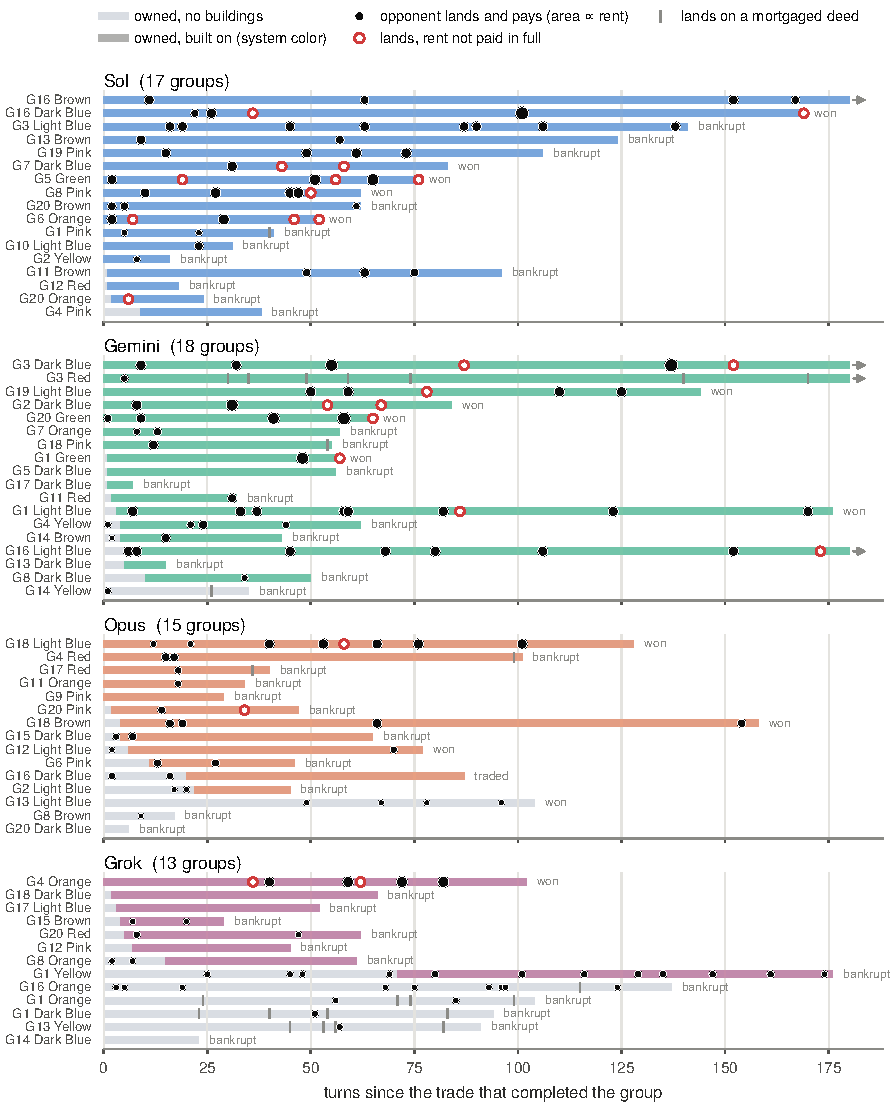
\includegraphics[width=\linewidth,height=0.80\textheight,keepaspectratio]{fig_timeline.pdf}
\caption{Every color group completed by trade, from the completing trade to the end of the episode. Rows are ordered by how soon the owner built. Episodes longer than 180 turns are clipped at the arrow. The label at the right says how the episode ended.}
\label{fig:timeline}
\end{figure}

\begin{table}[H]
\centering\small
\begin{tabular}{@{}rrrrrrrrr@{}}
\toprule
& \multicolumn{4}{c}{Sol and Gemini} & \multicolumn{4}{c}{Opus and Grok}\\
\cmidrule(lr){2-5}\cmidrule(l){6-9}
Seed block & Groups & Landings & Rent & Per landing & Groups & Landings & Rent & Per landing\\
\midrule
\BlockRentRows
\bottomrule
\end{tabular}
\caption{Rent per opponent landing on trade-completed groups, by seed block.}
\label{tab:blockrent}
\end{table}

\begin{table}[H]
\centering\small
\begin{tabular}{@{}lrrrr@{}}
\toprule
& Debt & & & Eliminated with a\\
System & episodes & Paid & Eliminated & payment route\\
\midrule
\DebtRows
\bottomrule
\end{tabular}
\caption{Debt episodes by system. Payment routes for the three eliminations in the last column are inherited.}
\label{tab:debt}
\end{table}

Of the \fact{debt.paid} payments, \fact{debt.paid-composition.mortgage-only} used mortgages only, \fact{debt.paid-composition.sales-only} building sales only and \fact{debt.paid-composition.both} both. Of the \fact{debt.eliminated} eliminations, \fact{debt.eliminated-after-some-liquidation} followed at least one liquidation action in the same episode and \fact{debt.eliminated-after-building-sale} followed a building sale. The median trade-completed group is landed on \fact{conv.trade-groups.median-landings-per-group} times. Seller outcomes in Table~\ref{tab:sellers} are stable to the building window. With a four-turn window \fact{conv.seller-conversion.sensitivity-window-4.all-one-sided.built-after-sale.seller-won} of \fact{conv.seller-conversion.sensitivity-window-4.all-one-sided.built-after-sale.n} builders and \fact{conv.seller-conversion.sensitivity-window-4.all-one-sided.no-construction-after-sale.seller-won} of \fact{conv.seller-conversion.sensitivity-window-4.all-one-sided.no-construction-after-sale.n} others won. With a twelve-turn window the counts are \fact{conv.seller-conversion.sensitivity-window-12.all-one-sided.built-after-sale.seller-won} of \fact{conv.seller-conversion.sensitivity-window-12.all-one-sided.built-after-sale.n} and \fact{conv.seller-conversion.sensitivity-window-12.all-one-sided.no-construction-after-sale.seller-won} of \fact{conv.seller-conversion.sensitivity-window-12.all-one-sided.no-construction-after-sale.n}. Among sellers with under \$100, \fact{conv.seller-conversion.sensitivity-window-4.seller-under-100.built-after-sale.seller-won} of \fact{conv.seller-conversion.sensitivity-window-4.seller-under-100.built-after-sale.n} builders won with the four-turn window and \fact{conv.seller-conversion.sensitivity-window-12.seller-under-100.built-after-sale.seller-won} of \fact{conv.seller-conversion.sensitivity-window-12.seller-under-100.built-after-sale.n} with the twelve-turn window, and no seller who did not build won under either.

\section{Estates and cohort}
\label{app:estates}

\begin{table}[H]
\centering\footnotesize
\begin{tabularx}{\linewidth}{@{}rrllrrrL{0.14\linewidth}Yl@{}}
\toprule
& & First & First & \multicolumn{3}{c}{Creditor before the estate} & Creditor's & Estate deeds &\\
\cmidrule(lr){5-7}
G & Turn & out & creditor & share & rank & rent rank & built groups & (complete groups) & Winner\\
\midrule
\EstateRows
\bottomrule
\end{tabularx}
\caption{Positions at the first liquidation menu of the debt that ends in each game's first elimination. Share and rank refer to total assets, and rent rank to rent received so far. With rent received as the measure of who was ahead, the first creditor leads in \fact{estate.first-creditor-leads-rent-received} games.}
\label{tab:estates}
\end{table}

\begin{table}[H]
\centering\small
\begin{tabular}{@{}lrrrr@{}}
\toprule
Completing acquisition & Episodes & Eventual winner & With any rent & Rent received\\
\midrule
\RouteRows
\bottomrule
\end{tabular}
\caption{How color groups were completed. Winner status comes from the same games, so the column describes concentration and no effect on winning.}
\label{tab:routes}
\end{table}

\begin{table}[H]
\centering\small
\begin{tabular}{@{}rrrrlr@{}}
\toprule
Game & Seed block & Rotation & Turns & Winner & Winner's seat\\
\midrule
\CohortRows
\bottomrule
\end{tabular}
\caption{The cohort. Seeds by block are 751774554, 2506298840, 2573692901, 3648314310 and 2766649504. Rotations are cyclic, so the four rotations of a block cover 4 of the 24 possible seat orders.}
\label{tab:cohort}
\end{table}

\section{Controls and transcript provenance}
\label{app:transcripts}

Three further exchanges limit how the incidents should be read. They are context and enter no count.

\paragraph{A false premise is corrected and the offer accepted (G19).} Grok's applied call proposes Virginia and \$150 for States, with this message.
\TranscriptQuote{g19-d135-public}
Both deeds are pink. The private note on the same response retracts the offer, and the response text names a different action, ending the turn.
\TranscriptQuote{g19-d135-note}
\TranscriptQuote{g19-d136-public}
Sol corrects the color claim and accepts the terms. Accepting an offer need not mean accepting the proposer's account of it.

\paragraph{A false completion claim is corrected and a true one is refused (G11).} Sol offers Virginia for Grok's Pennsylvania and says Virginia completes Grok's pinks. It does not, because Sol also holds St.\ Charles.
\TranscriptQuote{g11-d256-public}
\TranscriptQuote{g11-d257-public}
\TranscriptQuote{g11-d258-public}
The second offer would complete Grok's pinks, and Grok still refuses because the trade completes Sol's greens.

\paragraph{A false obstacle follows a decision already made (G3).} With one house left in the bank, Grok tells Gemini that it cannot build, while its own note says that it can.
\TranscriptQuote{g3-d363-public}
\TranscriptQuote{g3-d363-note}
\TranscriptQuote{g3-d364-note}
Gemini had already chosen to hold before the message. A false statement followed by the behavior it urges does not show that the statement was relied on.

\paragraph{How quotations are produced.} A script reads each quoted field from the canonical decision file and writes the quotation, its label and a manifest entry with the file hash, line, field pointer, character span and field hash. No quotation is typed by hand. A label names the speaker, the channel, the game, the zero-based decision and the selected attempt, and says whether the card shows the full field or an excerpt. Bracketed ellipses mark omitted text. Errors in quotations are left as written. There are four channels. A public message and a private note are fields of the applied action. Assistant content is the text returned beside a tool call. The returned provider explanation is the provider's reasoning field. For public messages addressed to a counterparty, the manifest records the first later prompt of that player that contains the message. Of the \fact{d.quotes.cards} quotation cards, \fact{d.quotes.reused} repeat definitions checked in the earlier paper and match them character for character.

\section{Reproducibility, research assistance and authorship}
\label{app:repro}

The code and the twenty saved games are public at \url{https://github.com/KushagraBharti/MonopolyBench}. This draft is a later local artifact. It changes no game record, prompt, engine file or earlier manuscript, and it ran no game, engine call, replay or model call. Every table, figure, quotation and number in the text is generated by the scripts in the draft's \texttt{analysis} directory from the saved games and from the earlier ledgers named in Table~\ref{tab:reconcile}. A build fails if the text cites a number that the scripts do not produce.

The project uses LLM research assistants under human direction. In this round four assistants each wrote a complete paper independently before any cross-review. This draft was written by one of them, Claude Fable 5.2, which shares a developer with the evaluated Opus system. The assistant chose the analyses, the incidents and the framing after reading the records and the earlier reviews. The two semantic readings cited in Section~\ref{sec:attention} came from other assistant instances in earlier work. No human labeled any record for this paper, and no assistant is an author. The human author line is the project owner's decision.
